\chapter{Schwarzschild black hole}
\label{s:sch}
\index{Schwarzschild!black hole}

\minitoc

\section{Introduction}

After having discussed stationary black holes in Chap.~\ref{s:sta},
we examine here the simplest of them: the Schwarzschild black hole.
Let us recall that the prime importance of this object
in general relativity stems from the no-hair theorem (Sec.~\ref{s:sta:no-hair}),
which implies that any non-rotating black hole in an asymptotically flat
4-dimensional spacetime must be a Schwarzschild black hole.

\section{The Schwarzschild-(anti-)de Sitter solution}

\subsection{Vacuum Einstein equation with a cosmological constant}

Let us search for a static and spherically symmetric solution of the
Einstein equation (\ref{e:bas:Einstein_eq}) in a vacuum
4-dimensional spacetime $(\M,\w{g})$ with some arbitrary cosmological constant
$\Lambda$. Setting $\w{T}=0$ in Eq.~(\ref{e:bas:Einstein_eq}) yields
the equation to solve:
\be \label{e:sch:vac_Einstein_eq}
     \w{R} + \left(\Lambda - \frac{1}{2}\, R\right) \w{g} = 0 ,
\ee
$\w{R}$ being the Ricci tensor of $\w{g}$ and $R:=g^{\mu\nu} R_{\mu\nu}$ its
trace with respect to $\w{g}$, i.e. the so-called Ricci scalar
(cf. Sec.~\ref{s:bas:Ricci_tensor} in Appendix~\ref{s:bas}).
Let us first note that Eq.~(\ref{e:sch:vac_Einstein_eq}) implies a
constraint on $R$. Indeed the trace of Eq.~(\ref{e:sch:vac_Einstein_eq})
with respect to $\w{g}$ is
\[
    R + \left(\Lambda - \frac{1}{2}\, R\right) \times 4 = 0 ,
\]
hence
\be \label{e:sch:R_4Lamb}
    \encadre{R = 4\Lambda} .
\ee
In particular $R$ is constant.
Inserting this value back into (\ref{e:sch:vac_Einstein_eq}), we get
\be \label{e:sch:vac_Einstein_eq_Lamb}
    \encadre{ \w{R} = \Lambda \, \w{g} } .
\ee
Since this equation yields (\ref{e:sch:R_4Lamb}) as well, we conclude
that it is equivalent to (\ref{e:sch:vac_Einstein_eq}).

\subsection{Static and spherically symmetric metric} \label{s:sch:static_spher}

Let us assume that the spacetime $(\M,\w{g})$ is \defin{static}\index{static spacetime}:
the translation group $(\R,+)$ is a isometry group of $(\M,\w{g})$
(cf. Sec.~\ref{s:neh:symmetries}), with orbits that are timelike
(stationarity property) and hypersurface-orthogonal (staticity property, cf. Sec.~\ref{s:sta:staticity_thm}). Let us denote by $\w{\xi}$ the associated Killing vector
field (unique up to some constant rescaling), i.e. the generator of the
isometry group $(\R,+)$ (cf. Sec.~\ref{s:neh:symmetries}).

We may foliate $\M$ by a 1-parameter family of hypersurfaces
$\left(\Sigma_t\right)_{t\in\R}$, such that $\w{\xi}$ is normal to
all $\Sigma_t$'s and $t$ is a parameter associated to $\w{\xi}$:
\be \label{e:sch:xi_t}
    \w{\xi}(t) = 1
\ee
or equivalently,
\[
    \langle \dd t , \w{\xi} \rangle = 1.
\]

In addition to being static, we assume that $(\M,\w{g})$ is \defin{spherically symmetric},
i.e. that it is invariant under the action of the rotation group $\mathrm{SO}(3)$,
whose orbits are spacelike 2-spheres (cf. Sec.~\ref{s:neh:symmetries}).
Let $\Sp$ be some generic orbit 2-sphere. The static Killing vector field $\w{\xi}$
must be orthogonal to $\Sp$, otherwise the orthogonal projection of $\w{\xi}$
onto $\Sp$ would define some privileged directions on $\Sp$, which is incompatible
with spherical symmetry. The orthogonality of $\w{\xi}$ and $\Sp$ implies
that $\Sp\subset\Sigma_t$. Let $(x^a)=(\th,\ph)$ be spherical coordinates on
$\Sp$. The (Riemannian) metric $\w{q}$ induced by $\w{g}$ on $\Sp$ is given by
\be
    q_{ab}\, \D x^a\, \D x^b = r^2 \left( \D\th^2 + \sin^2\th\, \D\ph^2 \right) .
\ee
The positive coefficient $r^2$ in front of the standard spherical element must be
constant over $\Sp$, by virtue of spherical symmetry. The area of $\Sp$ is
then $A=4\pi r^2$. For this reason, $r$ is called the \defin{areal radius}\index{areal!radius}
of $\Sp$. Letting $\Sp$ vary, $r$ can be considered as a scalar field on
$\M$. If $\dd r \not = 0$, we may use it a coordinate. Since $\Sp\subset \Sigma_t$,
$(r,\th,\ph)$ is a coordinate system on each hypersurface $\Sigma_t$.
The set $(t,r,\th,\ph)$,
where $t$ is adapted to $\w{\xi}$ thanks to (\ref{e:sch:xi_t}), is then a
spacetime coordinate system and, by construction, the expression of the metric tensor
with respect to this system is
\be \label{e:sch:g_AB}
    g_{\mu\nu}\, \D x^\mu \, \D x^\nu = -A(r)\, \D t^2 + B(r)\, \D r^2 +
        r^2 \left( \D\th^2 + \sin^2\th\, \D\ph^2 \right) .
\ee
Note that in this coordinate system
\be
    \w{\xi} = \wpar_t
\ee
and that $g_{tt} = -A(r)$ and $g_{rr} = B(r)$ do not depend on $t$
as a result of the spacetime stationarity, while
$g_{tr} = g_{t\th} = g_{t\ph} = 0$ expresses the orthogonality of $\w{\xi}$
and $\Sigma_t$, i.e. the spacetime staticity.
The coordinates $(t,r,\th,\ph)$ are called \defin{areal coordinates}\index{areal!coordinates},
reflecting the fact that $r$ is the areal radius.

\subsection{Solving Einstein equation}

The Christoffel symbols of the metric (\ref{e:sch:g_AB}) with respect to the
areal coordinates are (cf. Sec.~\ref{s:sam:Kottler_solution} for the computation):
\be \label{e:sch:Christoffel_AB}
\begin{array}{l}
\displaystyle  \Gamma^t_{\ \, tr} = \Gamma^t_{\ \, rt} = \frac{1}{2A}\derd{A}{r}\qquad
\Gamma^r_{\ \, tt} = \frac{1}{2B}\derd{A}{r} \qquad
\Gamma^r_{\ \, rr} = \frac{1}{2B}\derd{B}{r} \qquad
\Gamma^r_{\ \, \th\th} = -\frac{r}{B} \\[2ex]
\displaystyle  \Gamma^r_{\ \, \ph\ph} = -\frac{r\sin^2\th}{B} \qquad
\Gamma^\th_{\ \, r\th} = \Gamma^\th_{\ \, \th r} = \frac{1}{r} \qquad
\Gamma^\th_{\ \, \ph\ph} = -\sin\th\cos\th \\[2ex]
\displaystyle \Gamma^\ph_{\ \, r\ph} = \Gamma^\ph_{\ \, \ph r} = \frac{1}{r} \qquad
\Gamma^\ph_{\ \, \th\ph} = \Gamma^\ph_{\ \, \ph\th} = \frac{1}{\tan\th} ,
\end{array}
\ee
the Christoffel symbols not listed above being zero.

The $tt$ component of the Einstein equation (\ref{e:sch:vac_Einstein_eq})
leads to (cf. Sec.~\ref{s:sam:Kottler_solution} for the computation)
\be \label{e:sch:EE_tt}
        r \derd{B}{r} - B + (1 - \Lambda r^2) B^2 = 0 ,
\ee
while the $rr$ component leads to
\be \label{e:sch:EE_rr}
        r \derd{A}{r} + A - (1 - \Lambda r^2) AB = 0 .
\ee
Finally, the $\th\th$ and $\ph\ph$ components lead to the same equation:
\be
    2  \frac{\D^2 A}{\D r^2} + \frac{2}{r} \derd{A}{r}
        - \frac{1}{B} \left( \derd{A}{r} + \frac{2A}{r} \right) \derd{B}{r}
        - \frac{1}{A} \left( \derd{A}{r} \right) ^2
        + 4 \Lambda  A B  = 0 .
\ee
All the other components of the Einstein equation (\ref{e:sch:vac_Einstein_eq})
are identically zero.

Adding Eq.~(\ref{e:sch:EE_tt}) multiplied by $A$ to
Eq.~(\ref{e:sch:EE_rr}) multiplied by $B$ yields
\[
    B \derd{A}{r} + A \derd{B}{r} = \derd{}{r}(AB) = 0 .
\]
The solution of this equation is obviously $A(r)B(r) = C$, where $C$ is a constant.
Without any loss of generality, we may choose $C=1$. Indeed, substituting
$C/B(r)$ for $A(r)$ in Eq.~(\ref{e:sch:g_AB}) results in
\[
    g_{\mu\nu}\, \D x^\mu \, \D x^\nu = -\frac{C}{B(r)}\, \D t^2 + B(r)\, \D r^2 +
        r^2 \left( \D\th^2 + \sin^2\th\, \D\ph^2 \right) .
\]
Assuming $C>0$, the change of variable $t' = \sqrt{C} t$, which is equivalent
to changing the stationary Killing vector from $\w{\xi}$ to
$\w{\xi}'=  1/\sqrt{C}\, \w{\xi}$,
yields
\[
    g_{\mu\nu}\, \D x^\mu \, \D x^\nu = -\frac{1}{B(r)}\, \D t'^2 + B(r)\, \D r^2 +
        r^2 \left( \D\th^2 + \sin^2\th\, \D\ph^2 \right) ,
\]
which is exactly the solution corresponding to $C=1$. Hence from now on,
we set $C=1$, i.e.
\be
    B(r) = \frac{1}{A(r)} .
\ee
Substituting this expression in Eq.~(\ref{e:sch:EE_rr}) yields an ordinary
differential equation for $A(r)$:
\[
    r \derd{A}{r} + A - 1 + \Lambda r^2 = 0 ,
\]
the solution of which is
\be
    A(r) = 1 - \frac{2 m}{r} - \frac{\Lambda}{3} \,  r^2 ,
\ee
where $m$ is a constant.
The general static and spherically symmetric solution of the vacuum
Einstein equation (\ref{e:sch:vac_Einstein_eq}) is therefore
\be \label{e:sch:Kottler_metric}
    \encadre{
        g_{\mu\nu}\, \D x^\mu \, \D x^\nu =
            -\left( 1 - \frac{2 m}{r} - \frac{\Lambda}{3} \,  r^2\right)\, \D t^2
            + \left( 1 - \frac{2 m}{r} - \frac{\Lambda}{3} \,  r^2\right) ^{-1}\, \D r^2+
        r^2 \left( \D\th^2 + \sin^2\th\, \D\ph^2 \right) }.
\ee
It is called the \defin{Kottler metric}\index{Kottler metric} (cf. the historical
note below).
The  \defin{Schwarzschild metric}\index{Schwarzschild!metric} is the
particular case $\Lambda=0$. If $\Lambda>0$,
(\ref{e:sch:Kottler_metric}) is called the
\defin{Schwarzschild-de Sitter metric}\index{Schwarzschild!de Sitter metric},
often abridged as \defin{Schwarzschild-dS metric}, while if $\Lambda<0$, it
is called the \defin{Schwarzschild-anti-de Sitter metric}\index{Schwarzschild!anti-de Sitter metric},
often abridged as \defin{Schwarzschild-AdS metric}\index{Schwarzschild!AdS metric}.

In the rest of this chapter, we will focuss on the Schwarzschild metric,
i.e. on the version $\Lambda=0$ of Eq.~(\ref{e:sch:Kottler_metric}):
\be \label{e:sch:Schwarz_metric_SD}
    \encadre{
        g_{\mu\nu}\, \D x^\mu \, \D x^\nu =
            -\left( 1 - \frac{2 m}{r} \right)\, \D t^2
            + \left( 1 - \frac{2 m}{r} \right) ^{-1}\, \D r^2 +
        r^2 \left( \D\th^2 + \sin^2\th\, \D\ph^2 \right) }.
\ee
The areal coordinates $(t,r,\th,\ph)$ are then called the
\defin{Schwarzschild-Droste coordinates}\index{Schwarzschild-Droste coordinates}\footnote{In the literature they are often referred to as simply
\defin{Schwarzschild coordinates}\index{Schwarzschild!coordinates}.}.

Since $A(r) = 1-2m/r$ and $B(r) = (1-2m/r)^{-1}$ for the Schwarzschild metric,
the non-vanishing Christoffel symbols (\ref{e:sch:Christoffel_AB}) become
\be \label{e:sch:Christoffel_SD}
\begin{array}{l}
\displaystyle  \Gamma^t_{\ \, tr} = \Gamma^t_{\ \, rt} = \frac{m}{r(r-2m)}\qquad
\Gamma^r_{\ \, tt} = \frac{m(r-2m)}{r^3} \qquad
\Gamma^r_{\ \, rr} =  - \frac{m}{r(r-2m)}\\[2ex]
\displaystyle \Gamma^r_{\ \, \th\th} = 2m-r \qquad  \Gamma^r_{\ \, \ph\ph} = (2m -r)\sin^2\th \qquad
\Gamma^\th_{\ \, r\th} = \Gamma^\th_{\ \, \th r} = \frac{1}{r} \\[2ex]
\displaystyle \Gamma^\th_{\ \, \ph\ph} = -\sin\th\cos\th \qquad \Gamma^\ph_{\ \, r\ph} = \Gamma^\ph_{\ \, \ph r} = \frac{1}{r} \qquad
\Gamma^\ph_{\ \, \th\ph} = \Gamma^\ph_{\ \, \ph\th} = \frac{1}{\tan\th} .
\end{array}
\ee

\begin{hist}
The Schwarzschild metric (\ref{e:sch:Schwarz_metric_SD}) is actually
the first non-trivial (i.e. different from Minkowski metric) solution
of Einstein equation ever found. It has been obtained by the
astrophysicist Karl Schwarzchild in the end of 1915 \cite{Schwa1916}, only a few weeks
after the publication of the articles funding general relativity by
Albert Einstein. It is also quite remarkable that
Schwarzschild found the solution while serving in the German army at the Russian
front. Unfortunately, he died from a rare skin disease a few month later.
The way Schwarzschild proceeded was quite different from that exposed above:
instead of the coordinates $(t,r,\th,\ph)$
named today after him, he used the coordinates
$(t,x^1,x^2,\ph)$ where $x^1 = r_*^3/3$, with $r_*^3 = r^3-8m^3$, and
$x^2 = -\cos\th$. Such a choice was made to enforce $\det(g_{\alpha\beta}) = -1$, a condition
prescribed by Einstein in an early version of general relativity, which had been presented on
18 November 2015 and on which Schwarzschild was working. Only in the final version, published on
25 November 2015, did Einstein relax the condition $\det(g_{\alpha\beta}) = -1$, allowing for full
covariance. Schwarzschild however
exhibited the famous line element (\ref{e:sch:Schwarz_metric_SD}), via what he
called the ``auxiliary quantity'' $r = (r_*^3 + 8m^3)^{1/3}$.
For him, the ``center'',  namely the location of the ``point mass'' generating the field,
was at $r_* = 0$, i.e. at $r=2m$.
Independently of Schwarzschild, Johannes Droste, then PhD student of
Hendrik Lorentz,
arrived at the solution (\ref{e:sch:Schwarz_metric_SD}) in May 1916 \cite{Drost1917}.
Contrary to Schwarzschild, Droste performed the computation with
a spherical coordinate system, $(t,\bar r, \th,\ph)$, yet distinct from
the standard ``Schwarzschild-Droste'' coordinates $(t,r,\th,\ph)$ by the fact that the radial
coordinate $\bar r$ was not chosen to be the areal radius, but instead a
coodinate for which $g_{\bar r\bar r} = 1$. At the end, by a change of
variable, Droste exhibited the line element (\ref{e:sch:Schwarz_metric_SD}).
The generalization to a non-vanishing cosmological constant, i.e.
Eq.~(\ref{e:sch:Kottler_metric}), has been obtained by
Friedrich Kottler in 1918 \cite{Kottl1918} and, independently, by
Hermann Weyl in 1919 \cite{Weyl1919}. We refer to Eisenstaedt's article
\cite{Eisen82} for a detailed account of the early history of the
Schwarzschild solution.
\end{hist}


\subsection{The Schwarzschild-Droste domain} \label{s:sch:SD_domain}

We immediately notice on (\ref{e:sch:Schwarz_metric_SD}) that the metric
components are singular at $r=0$ and $r=2m$. Accordingly, the Schwarzschild-Droste coordinates $(t,r,\th,\ph)$ cover the following subset of $\M$, which we call the
\defin{Schwarzschild-Droste domain}\index{Schwarzschild-Droste!domain}:
\begin{subequations}
\begin{align}
    \M_{\rm SD} & :=  \M_{\rm I} \cup \M_{\rm II} , \\
    \M_{\rm I} & :=  \R\times(2m,+\infty)\times\SS^2 ,\\
    \M_{\rm II} & :=  \R\times(0,2m)\times\SS^2 ,
\end{align}
\end{subequations}
with the coordinate $t$ spanning $\R$, the coordinate $r$ spanning $(2m,+\infty)$
on $\M_{\rm I}$ and $(0,2m)$ on $\M_{\rm II}$, and the coordinates $(\th,\ph)$
constituting a standard spherical chart of $\SS^2$.
Note that $\M_{\rm SD}$ is a disconnected open subset of the full spacetime
manifold $\M$ (to be specified later), whose connected components are
$\M_{\rm I}$ and $\M_{\rm II}$.

\begin{remark}
To cover entirely $\SS^2$ in a regular way, one needs a second chart, in
addition to $(\th,\ph)$; this is related to the standard singularities of
spherical coordinates at $\th=0$ and $\th=\pi/2$. It is fully understood
that the metric $\w{g}$, as expressed by (\ref{e:sch:Schwarz_metric_SD}), is
fully regular on $\SS^2$. The fact that $\det(g_{\alpha\beta}) = -r^2\sin^2\th$ is zero
at $\th=0$ and $\th=\pi/2$ reflects merely the coordinate singularity
of the $(\th,\ph)$ chart there. We shall not discuss this coordinate singularity
any further.
\end{remark}

A first property of the Schwarzschild metric is that $\M_{\rm I}$ has an
asymptotically flat end: it is clear on (\ref{e:sch:Schwarz_metric_SD})
that the metric $\w{g}$ tends to Minkowski metric (\ref{e:glo:Mink_metric_spher})
when $r\rightarrow +\infty$.

Besides, in region $\M_{\rm II}$, we notice on (\ref{e:sch:Schwarz_metric_SD})
that $g_{tt} > 0$. Since $g_{tt} = \w{g}(\wpar_t,\wpar_t)$, this implies
that the Killing vector field $\w{\xi} = \wpar_t$ is spacelike. Hence,
$(\M_{\rm II},\w{g})$ is not static, in the sense defined in
Sec.~\ref{s:sch:static_spher}: the translation group $(\R,+)$ is still an
isometry group of $(\M_{\rm II},\w{g})$, but its orbits are spacelike curves.
We note that $g_{rr} < 0$ in $\M_{\rm II}$, so that the
metric (\ref{e:sch:Schwarz_metric_SD}) keeps a Lorentzian signature,
as it should!
In other words, in $\M_{\rm II}$, $t$ becomes a space coordinate and
$r$ a time coordinate. Accordingly, the axes of the light cones
in Fig.~\ref{f:sch:rad_null_geod} are horizontal lines for $r<2m$.

%%%%%%%%%%%%%%%%%%%%%%%%%%%%%%%%%%%%%%%%%%%%%%%%%%%%%%%%%%%%%%%%%%%%%%%%%%%%%%%

\section{Radial null geodesics and Eddington-Finkelstein coordinates}

\subsection{Radial null geodesics}
\label{s:sch:rad_null_geod}

Let us search for the null geodesics of the Schwarzschild metric
(\ref{e:sch:Schwarz_metric_SD}) that are radial, i.e. along which
$\th=\mathrm{const}$ and $\ph=\mathrm{const}$. They are found by
setting  $\D\th=0$ and $\D\ph=0$
in (\ref{e:sch:Schwarz_metric_SD})
and searching for $\D s^2 = g_{\mu\nu}\, \D x^\mu \, \D x^\nu = 0$:
\be \label{e:sch:radial_null}
    \D s^2 = 0 \iff \D t^2 = \frac{\D r^2}{\left( 1 - \frac{2m}{r} \right) ^2} .
\ee
Hence the radial null geodesics are governed by
\be
    \D t = \pm \frac{\D r}{ 1 - \frac{2m}{r} } .
\ee
This equation is easily integrated:
\be
    t = \pm r \pm 2 m \ln \left| \frac{r}{2m} - 1 \right| + \mathrm{const} .
\ee
We have thus two families of curves, one for each choice
of sign in $\pm$:

\begin{figure}
\centerline{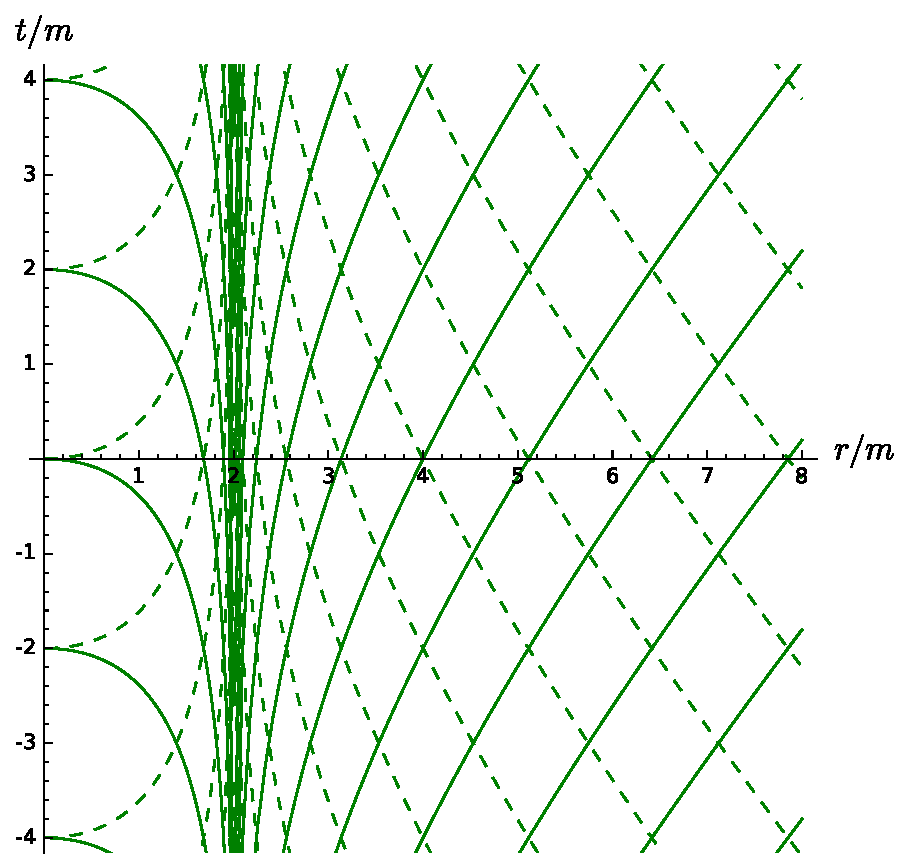
\includegraphics[width=0.6\textwidth]{sch_rad_null_geod.pdf}}
\caption[]{\label{f:sch:rad_null_geod} \footnotesize
Radial null geodesics of Schwarzschild spacetime, plotted in terms
of Schwarzschild-Droste coordinates $(t,r)$: the solid (resp. dashed) lines
correspond to outgoing (resp. ingoing) geodesics, as given by Eq.~(\ref{e:sch:outgoing_null_geod})
(resp. Eq.~(\ref{e:sch:ingoing_null_geod})). The interiors of some future light
cones are depicted in yellow.}
\end{figure}

\begin{itemize}
\item the \defin{outgoing radial null geodesics}\index{outgoing!null geodesic}, whose
equation is
\be \label{e:sch:outgoing_null_geod}
    t = r + 2 m \ln \left| \frac{r}{2m} - 1 \right| + u ,
\ee
where $u$ is a constant;
\item  the \defin{ingoing radial null geodesics}\index{ingoing!null geodesic}, whose
equation is
\be \label{e:sch:ingoing_null_geod}
    t = - r - 2 m \ln \left| \frac{r}{2m} - 1 \right| + v ,
\ee
where $v$ is a constant.
\end{itemize}

By introducing the \defin{tortoise coordinate}\index{tortoise coordinate}
\be \label{e:sch:def_tortoise}
    r_* := r + 2 m \ln \left| \frac{r}{2m} - 1 \right| ,
\ee
one may rewrite the above equations as
\bea
    &  & t = r_* + u \\
    &  & t = -r_* + v . \label{e:sch:v_advanced_tortoise}
\eea
The parameter $u$ appears then as a
\emph{retarded time}\index{retarded!time}\index{time!retarded --}:
$u = t - r_*$ and $v$ as an
\emph{advanced time}\index{advanced!time}\index{time!advanced --}: $v = t + r_*$.

Strictly speaking, we have found radial null \emph{curves} only, i.e. solutions of
Eq.~(\ref{e:sch:radial_null}). Since not all null curves
are geodesics\footnote{A famous counterexample is the helix in Minkowski
spacetime defined in terms of Minkowskian coordinates $(t,x,y,z)$ by $x = a\cos(t/a)$, $y = a\sin(t/a)$, $z=0$,
where $a$ is a positive constant. It is a null curve, but not a null geodesic.}, there remains to prove that the curves defined
by (\ref{e:sch:outgoing_null_geod}) and (\ref{e:sch:ingoing_null_geod})
obey the geodesic equation\index{geodesic!equation}:
\be \label{e:sch:geod_eqn}
    \frac{\D^2 x^\alpha}{\D \lambda^2} + \Gamma^\alpha_{\ \, \mu\nu}
        \derd{x^\mu}{\lambda} \derd{x^\nu}{\lambda} = 0 ,
\ee
where $\lambda$ is an affine parameter.
Let us check that (\ref{e:sch:geod_eqn}) is satisfied by choosing $\lambda=r$.
For the curves defined by (\ref{e:sch:outgoing_null_geod}), we have
\[
    x^\alpha(r) = \left( r + 2 m \ln \left| \frac{r}{2m} - 1 \right| + u,\ r,\  \th,\  \ph \right) .
\]
Hence
\[
    \derd{x^\alpha}{r} = \left( \frac{r}{r-2m}, 1, 0, 0 \right)
    \qquad\mbox{and}\qquad
    \frac{\D^2 x^\alpha}{\D r^2} = \left( - \frac{2m}{(r-2m)^2}, 0, 0, 0 \right) .
\]
Given the Christoffel symbols (\ref{e:sch:Christoffel_SD}), it is then a
simple exercice to show that Eq.~(\ref{e:sch:geod_eqn}) is satisfied.
The same property holds for the family (\ref{e:sch:ingoing_null_geod}). Hence
we conclude
\begin{greybox}
The radial null geodesics in the Schwarzschild-Droste domain are ruled by
Eqs.~(\ref{e:sch:outgoing_null_geod})-(\ref{e:sch:ingoing_null_geod}).
Moreover the areal radius $r$ is an affine parameter along them.
\end{greybox}

The two families of radial null geodesics are depicted in
Fig.~\ref{f:sch:rad_null_geod}.
The singularity of Schwarzschild-Droste coordinates at $r=2m$
is clearly apparent on this figure.


\begin{remark}
Despite their name, gedeosics of the outgoing family are actually
\emph{ingoing} in the region $r<2m$, in the sense that
$r$ is decreasing along them when moving towards the future. Indeed,
as noticed in Sec.~\ref{s:sch:SD_domain},
for $r<2m$, $r$ is the timelike coordinate of the system $(t,r,\th,\ph)$,
with $-\wpar_r$ oriented towards the future (cf. the ``tilted'' light cone
in Fig.~\ref{f:sch:rad_null_geod}).
\end{remark}

\subsection{Eddington-Finkelstein coordinates} \label{s:sch:EF_coord}

The parameter $v$ introduced in Eq.~(\ref{e:sch:ingoing_null_geod}) can be
seen as a label for the ingoing radial null geodesics: each of these curves is
entirely identified by the data $(v,\th,\ph)$, which remains fixed along it.
Let us promote $v$ to a spacetime coordinate, instead of $t$, i.e. let us
consider the coordinate system $(v,r,\th,\ph)$ with the relation to
Schwarzschild-Drostes coordinates $(t,r,\th,\ph)$ governed by Eq.~(\ref{e:sch:ingoing_null_geod}):
\be \label{e:sch:v_t_r}
     v = t + r + 2 m \ln \left| \frac{r}{2m} - 1 \right| .
\ee
It follows immediately that
\[
    \D v = \D t + \D r + \frac{\D r}{r/2m - 1} = \D t + \frac{\D r}{1 - 2m/r} ,
\]
i.e.
\[
    \D t = \D v -  \frac{\D r}{1 - 2m/r} .
\]
Taking the square gives
\[
    \D t^2 = \D v^2 - \frac{2}{1 - 2m/r} \, \D v \, \D r + \frac{1}{(1 - 2m/r)^2}\, \D r^2 .
\]
Substituting this expression for $\D t^2$ in Eq.~(\ref{e:sch:Schwarz_metric_SD})
yields the metric components with respect to the coordinates
$({\hat x}^\alpha) := (v,r,\th,\ph)$:
\be \label{e:sch:Schwarz_metric_NIEF}
    \encadre{
        {\hat g}_{\mu\nu}\, \D {\hat x}^\mu \, \D {\hat x}^\nu =
            -\left( 1 - \frac{2 m}{r} \right)\, \D v^2
            + 2 \, \D v \, \D r
        + r^2 \left( \D\th^2 + \sin^2\th\, \D\ph^2 \right) }.
\ee
The coordinates $({\hat x}^\alpha) = (v,r,\th,\ph)$ are called the
\defin{null ingoing Eddington-Finkelstein (NIEF) coordinates}\index{Eddington-Finkelstein!coordinates}\index{null!ingoing Eddington-Finkelstein coordinates}\index{NIEF}. The qualifier \emph{null} stems from the fact that
$r$ is a null coordinate in this system, i.e. the vector $\wpar_r$ of the coordinate
basis associated with $(v,r,\th,\ph)$ is a null
vector, as it follows from ${\hat g}_{rr}=0$ in Eq.~(\ref{e:sch:Schwarz_metric_NIEF}).

To deal with a ``standard'' time $+$ space coordinate system instead of a null one, let us set
\be  \label{e:sch:ti_v_r}
    \encadre{\ti := v - r} \iff \encadre{v = \ti + r}
\ee
and define the \defin{ingoing Eddington-Finkelstein (IEF) coordinates}\index{Eddington-Finkelstein!coordinates}\index{ingoing!Eddington-Finkelstein!coordinates}\index{IEF}
to be
\be
    (\tilde{x}^\alpha) := (\ti, r, \th,\ph) .
\ee

\begin{remark}
From (\ref{e:sch:ti_v_r}), $v$ appears as the ``time'' $\ti$ ``advanced'' by
$r$\index{advanced!time}\index{time!advanced --}, while
from (\ref{e:sch:v_advanced_tortoise}), $v$ is the ``time'' $t$ ``advanced''
by $r_*$.
\end{remark}

The relation between the ingoing Eddington-Finkelstein coordinates
$(\ti, r, \th,\ph)$
and the Schwarzschild-Droste ones $(t,r,\th,\ph)$ is obtained by combining
Eqs.~(\ref{e:sch:v_t_r}) and (\ref{e:sch:ti_v_r}):
\be \label{e:sch:ti_t_r}
     \encadre{\ti = t + 2 m \ln \left| \frac{r}{2m} - 1 \right| } .
\ee
The hypersurfaces $t=\mathrm{const}$ are plotted in Fig.~\ref{f:sch:SD_slices},
in terms of the IEF coordinates.

\begin{figure}
\centerline{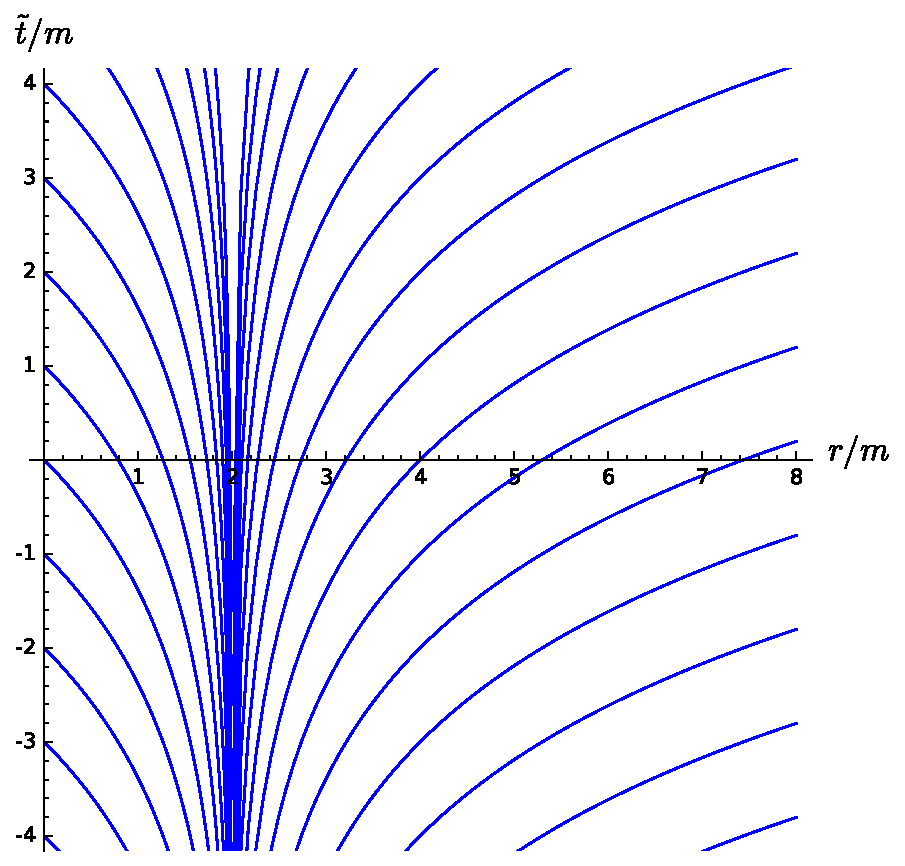
\includegraphics[width=0.6\textwidth]{sch_SD_slices.pdf}}
\caption[]{\label{f:sch:SD_slices} \footnotesize
Hypersurfaces of constant Schwarzschild-Droste coordinate $t$, drawn in term
of the ingoing Eddington-Finkelstein coordinates $(\ti,r)$. Since the dimensions
along $\th$ and $\ph$ are not represented, these 3-dimensional surfaces appear
as curves.}
\end{figure}

From (\ref{e:sch:ti_v_r}), we have $\D v = \D\ti + \D r$. Substituting
into (\ref{e:sch:Schwarz_metric_NIEF}) yields
\be \label{e:sch:Schwarz_metric_EF}
    \encadre{
        \tilde{g}_{\mu\nu}\, \D \tilde{x}^\mu \, \D \tilde {x}^\nu =
            -\left( 1 - \frac{2 m}{r} \right)\, \D \ti^2
            + \frac{4m}{r} \, \D \ti \, \D r
            + \left( 1 + \frac{2 m}{r} \right)\, \D r^2
        + r^2 \left( \D\th^2 + \sin^2\th\, \D\ph^2 \right) }.
\ee
We check that $\tilde{g}_{\ti\ti} < 0$ in $\M_{\rm I}$, hence $\ti$ is
a timelike coordinate there.
In $\M_{\rm II}$, $\tilde{g}_{\ti\ti} > 0$, so that $\ti$ becomes spacelike
there, as for the Schwarzschild-Droste coordinate $t$ (cf. Sec.~\ref{s:sch:SD_domain}).
However, we have $\tilde{g}_{rr} = 1+2m/r > 0$ everywhere, so that $r$ remains a spacelike coordinate (for the IEF system) in
$\M_{\rm II}$, contrary to what happens within the Schwarzschild-Droste coordinates
(cf. Sec.~\ref{s:sch:SD_domain}).

\begin{remark}
The above example shows that the property of being timelike, null or spacelike
is not intrinsic to a given coordinate (here $r$). It is instead a property
of the whole coordinate system under consideration. This is understandable
since $r$ spacelike means that the line along which $r$ varies while the
three other coordinates $(x^0,x^2,x^3)$ are kept constant is a spacelike curve.
For the Schwarzschild-Droste system $(x^0,x^2,x^3) = (t,\th,\ph)$,
while for the NIEF system
$(x^0,x^2,x^3) = (v,\th,\ph)$ and for
the IEF system $(x^0,x^2,x^3) = (\ti,\th,\ph)$.
Hence the three sets of $r$-lines differ.
Equivalently, the coordinate vectors $\wpar_r$
tangent to the three kinds of $r$-lines are different:
\[
    \left. \der{}{r} \right| _{t,\th,\ph} \not=
    \left. \der{}{r} \right| _{v,\th,\ph} \not=
    \left. \der{}{r} \right| _{\ti,\th,\ph} .
\]
\end{remark}
To avoid any ambiguity, we shall denote by $\wpar_{\tilde{r}}$ the
coordinate vector of the IEF frame and by
$\wpar_r$ the coordinate vector of the Schwarzschild-Droste frame:
\be
    \wpar_{\tilde{r}} := \left. \der{}{r} \right| _{\ti,\th,\ph}
    \qquad\mbox{and}\qquad
    \wpar_r := \left. \der{}{r} \right| _{t,\th,\ph} .
\ee
The relation between the two vectors is given by the chain rule:
\[
    \left. \der{}{r} \right| _{\ti,\th,\ph}  =
    \left. \der{}{t} \right| _{r,\th,\ph}
    \underbrace{ \left. \der{t}{r} \right| _{\ti,\th,\ph}}_{\left(1-\frac{r}{2m}\right)^{-1}}
  + \left. \der{}{r} \right| _{t,\th,\ph}
   \underbrace{\left. \der{r}{r} \right| _{\ti,\th,\ph}}_{1}
  + \left. \der{}{\th} \right| _{t,r,\ph}
  \underbrace{\left. \der{\th}{r} \right| _{\ti,\th,\ph}}_{0}
  + \left. \der{}{\ph} \right| _{t,r,\th}
  \underbrace{\left. \der{\ph}{r} \right| _{\ti,\th,\ph}}_{0} ,
\]
where (\ref{e:sch:ti_t_r}) has been used to evaluate
$\left. \dert{t}{r} \right| _{\ti,\th,\ph}$. Hence
\be
    \wpar_{\tilde{r}} = \wpar_r + \left(1-\frac{r}{2m}\right)^{-1} \, \wpar_t .
\ee

On the other hand, we deduce from (\ref{e:sch:ti_t_r}) that
\be
     \left. \der{}{\ti} \right| _{r,\th,\ph} = \left. \der{}{t} \right| _{r,\th,\ph} ,
\ee
which implies:
\be
    \wpar_{\ti} = \wpar_t .
\ee
In particular, the vector $\wpar_{\ti}$ of the IEF frame coincides with
the Killing vector $\w{\xi}$:
\be \label{e:sch:wparti_xi}
    \encadre{ \wpar_{\ti} = \w{\xi}} .
\ee
\begin{remark}
The result (\ref{e:sch:wparti_xi}) is not surprising since
the metric components (\ref{e:sch:Schwarz_metric_EF}) are independent from
$\ti$. This implies $\wpar_{\ti} = \alpha \w{\xi}$, where $\alpha$ is a constant.
Since $\ti \sim t$ when $r\rightarrow +\infty$, we conclude that $\alpha=1$.
\end{remark}

\begin{remark}
The IEF-coordinates line element (\ref{e:sch:Schwarz_metric_EF}) can be recast
in the following remarkable form:
\be \label{e:sch:Kerr_Schild}
    \tilde{g}_{\mu\nu}\, \D \tilde{x}^\mu \, \D \tilde {x}^\nu =
 \underbrace{- \D\ti^2 + \D r^2 + r^2  \left( \D\th^2 + \sin^2\th\, \D\ph^2 \right)}_{f_{\mu\nu} \, \D \tilde{x}^\mu \, \D \tilde {x}^\nu}
        + \underbrace{\frac{2m}{r} \left( \D\ti + \D r \right) ^2}_{k_\mu \D \tilde{x}^\mu \, k_\nu \D \tilde {x}^\nu} ,
\ee
where the $f_{\mu\nu}$'s are the components of the (flat) Minkowski metric expressed in
terms of the spherical coordinates $(\ti,r,\th,\ph)$ and the $k_\mu$'s are
the components of a 1-form dual to a null vector:
\[
    \uu{k} = \sqrt{\frac{2m}{r}} \, \dd (\ti + r) =
    \sqrt{\frac{2m}{r}} \, \dd v .
\]
The fact that $\w{k}$ is a null vector follows from
$g^{\mu\nu} k_\mu k_\nu = 0$, which is easily deduced from
$k_\mu = \sqrt{2m/r} (1, 1, 0, 0)$ and the expression (\ref{e:sch:inv_metric_EF})
of $g^{\mu\nu}$ below.
The line element (\ref{e:sch:Kerr_Schild}) is said to be of
\defin{Kerr-Schild form}\index{Kerr-Schild form}.
\end{remark}

\subsection{The Schwarzschild horizon} \label{s:sch:Schwarz_hor}

Contrary to the Schwarzschild-Droste components (\ref{e:sch:Schwarz_metric_SD}),
the metric components (\ref{e:sch:Schwarz_metric_EF}) are regular as
$r\rightarrow 2m$. In particular, their determinant is
\be
    \det\left( \tilde{g}_{\alpha\beta} \right) = - r^4\sin^2\th ,
\ee
which is never zero for $r\in(0,+\infty)$, except at the standard $\th=0$ and
$\th=\pi$ singularities of spherical coordinates.
This proves that
(\ref{e:sch:Schwarz_metric_EF}) defines a regular non-degenerate metric
on the whole \defin{ingoing Eddington-Finkelstein domain}\index{ingoing!Eddington-Finkelstein!domain}
\be
    \M_{\rm IEF} := \R\times(0,+\infty)\times\SS^2,
\ee
with the coordinate $\ti$ spanning $\R$, the coordinate $r$ spanning
$(0,+\infty)$ and the coordinates $(\th,\ph)$ forming a standard spherical
chart of $\SS^2$.
The components of the inverse metric with respect to the ingoing
Eddington-Finkelstein coordinates are
\be \label{e:sch:inv_metric_EF}
    {\tilde g}^{\alpha\beta} = \left( \begin{array}{cccc}
    - \left( 1 + \frac{2m}{r} \right) &  \frac{2m}{r} & 0 & 0 \\[1ex]
    \frac{2m}{r} & 1 - \frac{2m}{r} & 0 & 0 \\[1ex]
    0 & 0 & \frac{1}{r^2} & 0 \\[1ex]
    0 & 0 & 0 & \frac{1}{r^2\sin^2\th}
    \end{array} \right) .
\ee
In particular, the components ${\tilde g}^{\alpha\beta}$ are regular at $r=2m$.

The IEF domain is an extension of the Schwarzschild-Droste domain
introduced in Sec.~\ref{s:sch:SD_domain}:
\be
    \M_{\rm IEF} = \M_{\rm SD} \cup \Hor = \M_{\rm I} \cup \M_{\rm II} \cup \Hor ,
\ee
where $\Hor$ is the subset of $\M_{\rm IEF}$ defined by $r=2m$. Note that
$\Hor$ has the topology
\be
    \Hor \simeq \R\times\SS^2
\ee
and that $(\ti,\th,\ph)$ is a coordinate system on $\Hor$.
Actually $\Hor$ is nothing but what has been called the
\defin{Schwarzschild horizon}\index{Schwarzschild!horizon} in the examples
of Chaps.~\ref{s:def} and \ref{s:neh}. Indeed, the metric
(\ref{e:sch:Schwarz_metric_EF}) is nothing but
the metric (\ref{e:def:Schw_metric}) introduced in Example~\ref{x:def:Schw_hor}
of Chap.~\ref{s:def} (p.~\pageref{x:def:Schw_hor}), up to the change of notation $\ti \leftrightarrow t$ (compare (\ref{e:def:Schw_metric_inv}) and
(\ref{e:sch:inv_metric_EF}) as well).
We have thus the fundamental result,
the proof of which is given in Example~\ref{x:neh:Schwarz_KH} of Chap.~\ref{s:neh}
(p.~\pageref{x:neh:Schwarz_KH}):
\begin{greybox}
$\Hor$ is a Killing horizon, the null normal of which is $\w{\xi}$.
\end{greybox}
In particular, $\Hor$ is a null hypersurface, whose null geodesic generators
admit $\w{\xi} = \wpar_{\ti}$ as tangent vector. It is a non-expanding horizon,
whose area, as defined in Sec.~\ref{s:neh:invar_area}, is (cf. Example~\ref{x:neh:Schwarz_hor_area} of Chap.~\ref{s:neh}, p.~\pageref{x:neh:Schwarz_hor_area})
\be
    A=16\pi m^2 .
\ee
$\Hor$ is depicted in Fig.~\ref{f:def:Schwarz_horizon}.
We shall see in Sec.~\ref{s:sch:BH} that $\Hor$ is actually a
black hole event horizon in Schwarzschild spacetime.

\subsection{Coordinate singularity vs. curvature singularity}
\label{s:sch:singularities}

The above considerations show that the divergence of the metric
component $g_{rr}$ in (\ref{e:sch:Schwarz_metric_SD}) when $r\rightarrow 2m$
reflects a pathology of Schwarzschild-Droste coordinates and not a singularity
in the metric tensor $\w{g}$ by itself: $(\M_{\rm IEF}, \w{g})$ is perfectly
regular spacetime, including at $r=2m$.
The bad behaviour of of Schwarzschild-Droste coordinates is obvious in Fig.~\ref{f:sch:SD_slices}: the hypersurfaces
$t=\mathrm{const}$ fail to provide a regular slicing of spacetime.
This pathology is called a
\defin{coordinate singularity}\index{coordinate!singularity}\index{singularity!coordinate --}, since it is intrinsic a given coordinate system
(here the Schwarzschild-Droste one).

Another pathology appears in the metric components in both the Schwarzschild-Droste coordinates and the ingoing Eddington-Finkelstein ones: $g_{tt}$ and $\tilde{g}_{\ti\ti}$ diverge when $r\rightarrow 0$. This type of singularity
cannot be removed by a coordinate transformation. Indeed the
\defin{Kretschmann scalar}\index{Kretschmann scalar}, defined as the
following ``square'' of the Riemann curvature tensor
\be \label{e:sch:def_Kretschmann}
    K := R_{\mu\nu\rho\sigma} R^{\mu\nu\rho\sigma} ,
\ee
is (cf. Appendix~?? for the computation})
\be
    K = \frac{48 m^2}{r^6} .
\ee
Hence $K\rightarrow +\infty$ when $r\rightarrow 0$. Since $K$ is a scalar
field, its value is independent of any coordinate system used to express it.
Hence the divergence of $K$ reflects a pathology of the Riemann tensor
per se: it is called a
\defin{curvature singularity}\index{curvature!singularity}\index{singularity!curvature --}.


\begin{hist}
Eddington-Finkelstein coordinates have been introduced by
Arthur Eddington in 1924 \cite{Eddin1924}. More precisely, Eddington
introduced the \emph{outgoing} version of these coordinates,
while we have focussed above on the \emph{ingoing} version. Indeed
Eddington's Eq.~(2) is $\ti = t - 2m \ln(r-m)$, which mainly differs from
our Eq.~(\ref{e:sch:ti_t_r}) by the minus sign in front of the logarithm\footnote{The other differences with (\ref{e:sch:ti_t_r}) are a constant additive term
and a misprint in Eddington's formula: the term $\ln(r-m)$ should be replaced
by $\ln(r-2m)$.},
which means that Eddington's time coordinate is actually $\ti = u + r$, instead of
$\ti = v - r$ (our Eq.~(\ref{e:sch:ti_v_r})). Eddington used his transformation
to get the Kerr-Schild form (\ref{e:sch:Kerr_Schild}) of Schwarzschild metric,
with $(\D \ti + \D r)^2$ replaced by $(\D \ti - \D r)^2$ due to the change
ingoing $\leftrightarrow$ outgoing. For a modern reader, it is quite surprising
that Eddington did not point out that the metric components w.r.t. $(\ti,r,\th,\ph)$
are regular at $r=2m$. Actually the main purpose of Eddington's article
\cite{Eddin1924} was elsewhere, in the comparison of general relativity to an alternative theory proposed in 1922 by the mathematician Alfred N. Whitehead
(see e.g. \cite{GibboW08}).
Only in 1958 did David Finkelstein reintroduce the Eddington transformation
to demonstrate that the Schwarzschild metric is analytic over the whole domain
$r\in(0,+\infty)$ \cite{Finke58}. Meanwhile the regularity of Schwarzschild metric
at $r=2m$ had been proved by Georges Lemaître in 1932 \cite{Lemai32}, by means of
another coordinate system (see \cite{Eisen93} for a detailed discussion).
\end{hist}

\begin{remark}
In the literature, the terminology \emph{Eddington-Finkelstein coordinates}
is often used for the coordinates $(v,r,\th,\ph)$ (or $(u,r,\th,\ph)$),
i.e. for what we have called the \emph{null Eddington-Finkelstein coordinates},
and the regularity of the metric tensor at $r=2m$ is demonstrated by
considering the components (\ref{e:sch:Schwarz_metric_NIEF}).
However, neither
Eddington \cite{Eddin1924} nor Finkelstein \cite{Finke58}
considered this null version: they used coordinates $(\ti,r,\th,\ph)$, where
$\ti$ is timelike and they exhibited (the outgoing version of) the
metric components (\ref{e:sch:Schwarz_metric_EF}).
Hence our terminology is more faithfull to history. Moreover, focussing on
$(v,r,\th,\ph)$ may give the false impression to a novice reader that it is
necessary to introduce some null coordinate to establish the regularity
of the metric tensor at $r=2m$, while the timelike coordinate $\ti$
does the job very well.
\end{remark}

\begin{figure}
\centerline{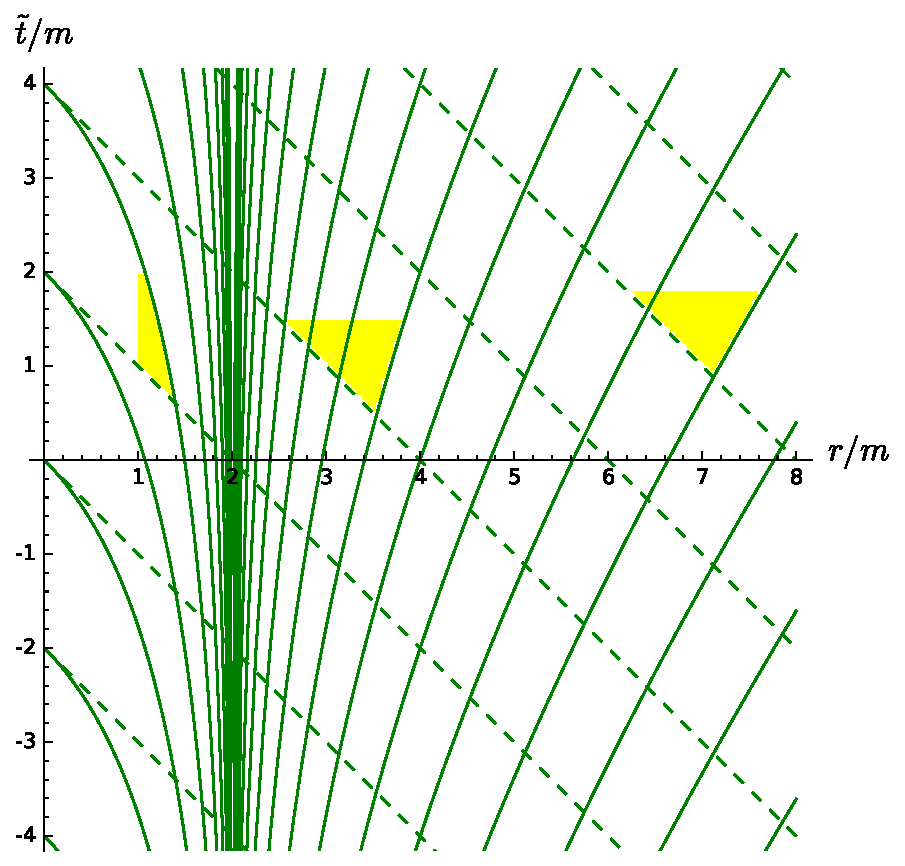
\includegraphics[width=0.6\textwidth]{sch_rad_null_geod_EF.pdf}}
\caption[]{\label{f:sch:rad_null_geod_EF} \footnotesize
Radial null geodesics of Schwarzschild spacetime, plotted in terms
of ingoing Eddington-Finkelstein coordinates $(\ti,r)$: the solid (resp. dashed) lines
correspond to outgoing (resp. ingoing) geodesics, as given by Eq.~(\ref{e:sch:outgoing_null_geod_EF})
(resp. Eq.~(\ref{e:sch:ingoing_null_geod_EF})). The interiors of some future light
cones are depicted in yellow.}
\end{figure}

\subsection{Radial null geodesics in terms of the Eddington-Finkelstein coordinates}

By construction, the equation of the ingoing radial null geodesics
in terms of the IEF coordinates is very simple:
\be \label{e:sch:ingoing_null_geod_EF}
    \ti = - r + v ,
\ee
where the constant $v\in \R$ labels the geodesic.
The equation of the outgoing radial null geodesics is obtained
by combining (\ref{e:sch:outgoing_null_geod}) and (\ref{e:sch:ti_t_r}):
\be \label{e:sch:outgoing_null_geod_EF}
    \ti = r + 4 m \ln \left| \frac{r}{2m} - 1 \right| + u ,
\ee
where the constant $u\in \R$ labels the geodesic.
The radial null geodesics are depicted in Fig.~\ref{f:sch:rad_null_geod_EF}
in terms of the IEF coordinates. We note that, contrary to Fig.~\ref{f:sch:rad_null_geod},
which was based on Schwarzschild-Drostes coordinates, in the region $r<2m$,
the future light cones point upwards. This reflects the fact that, in the IEF system,
$\ti$ is a timelike coordinate and $r$ a spacelike one.

%%%%%%%%%%%%%%%%%%%%%%%%%%%%%%%%%%%%%%%%%%%%%%%%%%%%%%%%%%%%%%%%%%%%%%%%%%%%%%%

\section{Black hole character} \label{s:sch:BH}

We have already seen in Sec.~\ref{s:sch:Schwarz_hor} that $\Hor$ is
a Killing horizon. In particular, it is a null hypersurface, and thereby a
one-way membrane (cf. Sec.~\ref{s:def:hor_as_null}).
Since $\Hor$ is the boundary of $\M_{\rm II}$, we conclude that no particle nor
electromagnetic signal may emerge from $\M_{\rm II}$
(this is pretty clear by looking to null geodesics on
Fig.~\ref{f:sch:rad_null_geod_EF}). Hence, with respect to the ``outside''
world, represented by the asympotically flat region $\M_{\rm I}$,
$\M_{\rm II}$ is a black hole.

\begin{figure}
\centerline{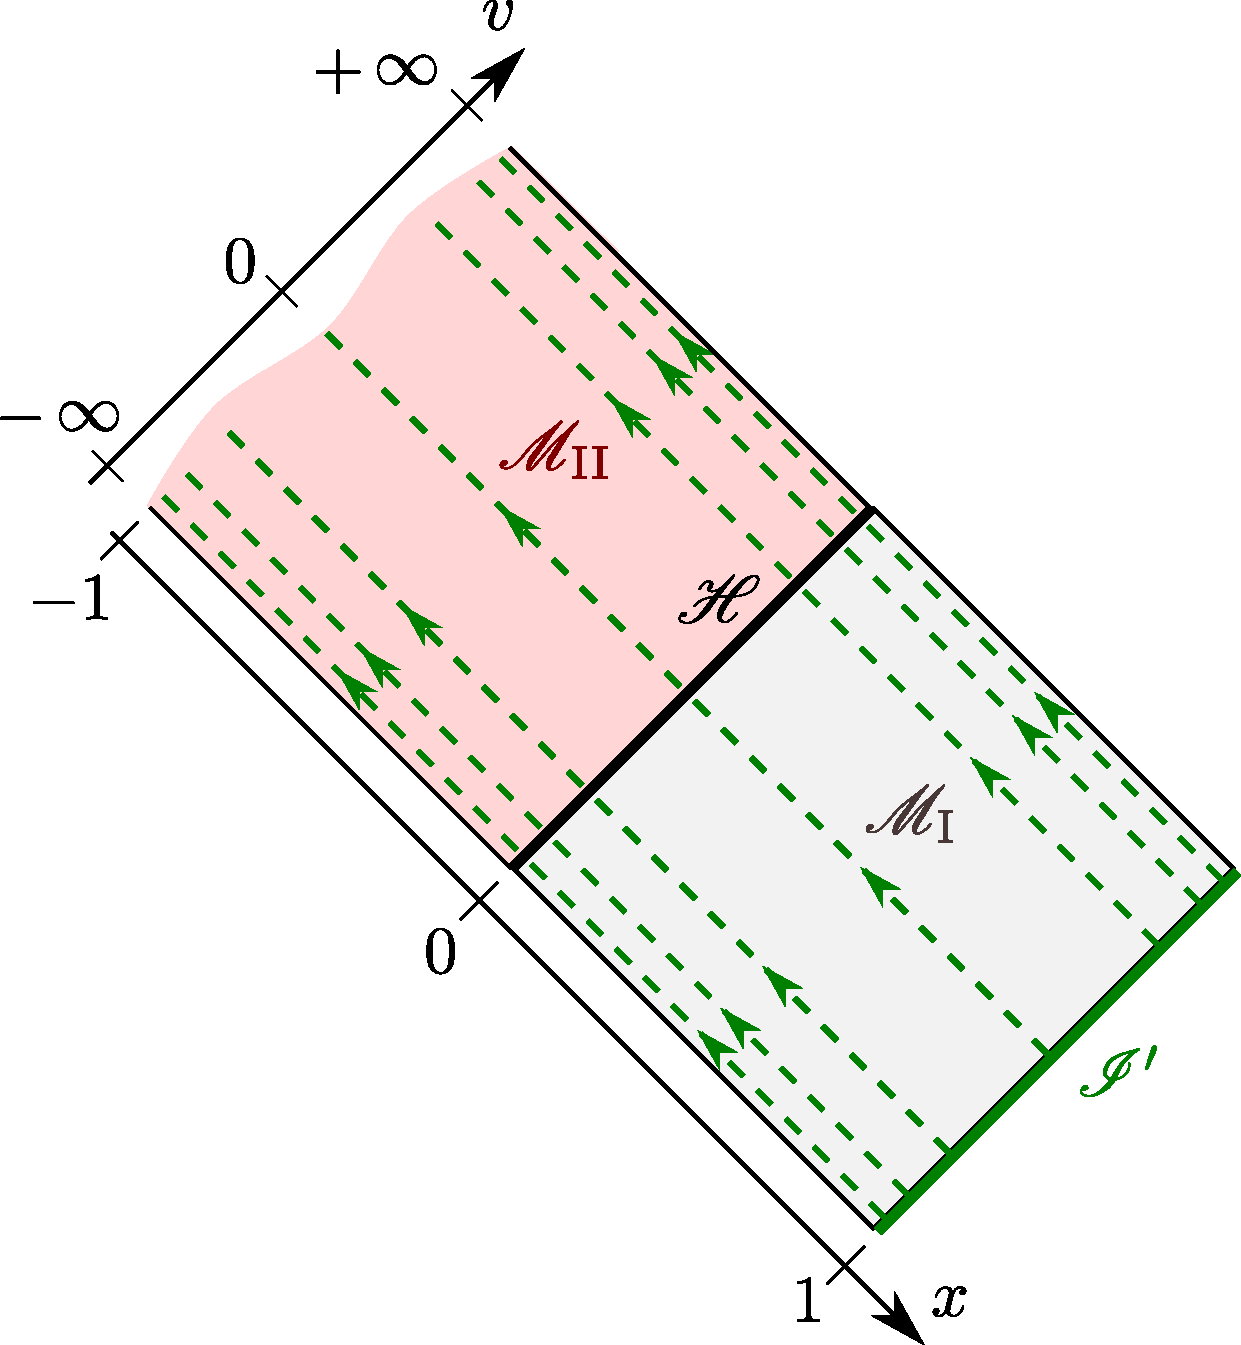
\includegraphics[width=0.5\textwidth]{sch_conf_compl1.pdf}}
\caption[]{\label{f:sch:conf_compl1} \footnotesize
Manifold with boundary
$\M' = \M_{\rm II}\cup\Hor\cup\M_{\rm I}\cup\scri'$, drawn in terms of
the coordinates $x$ and (a compactified version of) $v$.
The dashed lines are the ingoing radial null geodesics (as in Fig.~\ref{f:sch:rad_null_geod_EF}), the arrows marking the future orientation.}
\end{figure}


It would be satisfactory though to check that $\M_{\rm II}$ fulfills the
formal definition of a black hole region that we have given in
Sec.~\ref{s:glo:def_BH}.
The first step is to define a conformal
completion at null infinity $(\tilde{\M},\w{\tilde{g}})$ of
the Schwarzschild spacetime $(\M, \w{g})$, which we define
as the largest set considered so far, i.e. the ingoing Eddington-Finkelstein
domain:
\be
    \M := \M_{\rm IEF} = \M_{\rm I} \cup \Hor \cup \M_{\rm II} .
\ee
To this aim, let us start form the null ingoing Eddington-Finkelstein
coordinates $({\hat x}^\alpha)=(v,r,\th,\ph)$ introduced in Sec.~\ref{s:sch:EF_coord}; they
cover entirely $\M$ and the metric tensor $\w{g}$
is expressed in terms of them by Eq.~(\ref{e:sch:Schwarz_metric_NIEF}).
Performing the change of coordinates
$({\hat x}^\alpha)=(v,r,\th,\ph)\mapsto ({x'}^\alpha) = (v,x,\th,\ph)$
with
\be \label{e:sch:x_r}
    x = 1 - \frac{2m}{r} \iff r = \frac{2m}{1-x}, \qquad x\in (-\infty, 1),
\ee
we deduce from (\ref{e:sch:Schwarz_metric_NIEF}) that
\be
        {g'}_{\mu\nu}\, \D {x'}^\mu \, \D {x'}^\nu =
            -x \, \D v^2
            +\frac{4 m}{(1-x)^2} \, \D v \, \D x
        + \frac{4 m^2}{(1-x)^2}  \left( \D\th^2 + \sin^2\th\, \D\ph^2 \right) .
\ee
Defining
\be \label{e:sch:Omega_x_r}
    \Omega := 1-x = \frac{2m}{r} ,
\ee
we may rewrite the metric tensor as
\be
    \w{g} = \Omega^{-2} \w{\tilde{g}} ,
\ee
with the conformal metric
\be \label{e:sch:tilde_g_x_v}
    {\tilde{g}'}_{\mu\nu}\, \D {x'}^\mu \, \D {x'}^\nu =
            - x(1-x)^2 \, \D v^2
            +4 m \, \D v \, \D x
        + 4 m^2 \left( \D\th^2 + \sin^2\th\, \D\ph^2 \right) .
\ee
Since $(v,x,\th,\ph)$ is a global coordinate system on $\M$
(up to the trivial coordinate singularities of $(\th,\ph)$), we can
identify $\M$ to the following open subset of $\R^2\times\SS^2$:
\be \label{e:sch:M_subset_R2_S2}
    \M = \R \times (-\infty,1) \times \SS^2,
\ee
with $v$ spanning $\R$, $x$ spanning $(-\infty,1)$ and $(\th,\ph)$
spanning $\SS^2$.
Then we can extend $\M$ to the manifold with boundary (cf. Sec.~\ref{s:bas:manif_boundary})
\be
    \M' :=  \R \times (-\infty,1] \times \SS^2 .
\ee
Notice the change $(-\infty,1) \rightarrow (-\infty,1]$ with respect
to (\ref{e:sch:M_subset_R2_S2}), which means
that $x=1$ is an allowed value on $\M'$; it defines the boundary of
$\M'$, $\scri'$ say.
According to (\ref{e:sch:x_r}),
$\scri'$ corresponds to $r\rightarrow +\infty$.
A schematic view of the manifold $\M'$ is
provided in Fig.~\ref{f:sch:conf_compl1}.
We note that the conformal metric (\ref{e:sch:tilde_g_x_v}) can be extended
to the boundary $\scri'$, yielding a regular metric. Indeed, the determinant of
the metric components (\ref{e:sch:tilde_g_x_v}) is
\[
    \det\left({\tilde{g}'}_{\alpha\beta}\right) = - 64 m^6 \sin^2\th ,
\]
which does not vanish at $x=1$ (except at the trivial coordinate singularity
$\th=0$ or $\th=\pi$), showing that $\tilde{\w{g}}$ is a non-degenerate
symmetric bilinear form at $\scri'$ and hence a well defined metric on all
$\M'$.
Furthermore
we have $\Omega=0$ at $\scri'$ [set $x=1$ in Eq.~(\ref{e:sch:Omega_x_r})], as well as
\be
    \dd \Omega = - \dd x \not = 0 .
\ee
So, $(\M',\w{\tilde{g}})$ obeys all the conditions
listed in Sec.~\ref{s:glo:conf_compl} to form a \emph{conformal completion}
of $(\M,\w{g})$.
However, it is not a proper \emph{conformal completion at null infinity},
as defined in Sec.~\ref{s:glo:conf_compl} and required in the black hole
definition of Sec.~\ref{s:glo:def_BH}. Indeed any part of $\scri'$ is intersected by
a past-directed null geodesic (cf. Fig.~\ref{f:sch:conf_compl1}): a generic point of $\scri'$ has coordinates
$(v,x,\th,\ph) = (v_0,1,\th_0,\ph_0)$ and is the past end point of the
ingoing radial null geodesic defined by
$(v,\th,\ph) = (v_0,\th_0,\ph_0)$.
So $\scri'$ does not contain any future null infinity part ($\scri^+$). Actually,
we shall see below that $\scri'$ is entirely a past null infinity ($\scri^-$).
Therefore we shall extend $\M'$ to include some $\scri^+$ part.
To do this, we shall construct $\scri^+$ as the set of endpoints of the
\emph{outgoing} radial null geodesics in $\M_{\rm I}$. In terms of
the null ingoing Eddington-Finkelstein coordinates $(v,r,\th,\ph)$,
the equation of the
outgoing radial null geodesics is obtained by combining (\ref{e:sch:outgoing_null_geod_EF}) and (\ref{e:sch:ingoing_null_geod_EF}):
\be \label{e:sch:v_r_u}
    v = 2 r + 4 m \ln \left| \frac{r}{2m} - 1 \right| + u ,
\ee
where $u\in\R$ is a constant parameter along a given geodesic.
We notice that on $\M_{\rm I}$, we may use $(\check{x}^\alpha) = (u,r,\th,\ph)$ as a coordinate
system, naturally called the \defin{null outgoing Eddington-Finkelstein coordinates}\index{Eddington-Finkelstein!coordinates}\index{null!outgoing Eddington-Finkelstein coordinates}. Since (\ref{e:sch:v_r_u}) implies
\[
    \D v = \D u + \frac{2}{1-2m/r}\, \D r,
\]
we easily deduce from (\ref{e:sch:Schwarz_metric_NIEF}) the metric components
in these coordinates:
\be \label{e:sch:g_u_r}
        {\check{g}}_{\mu\nu}\, \D {\check{x}}^\mu \, \D {\check{x}}^\nu =
            -\left( 1 - \frac{2 m}{r} \right)\, \D u^2
            - 2 \, \D u \, \D r
        + r^2 \left( \D\th^2 + \sin^2\th\, \D\ph^2 \right) .
\ee
\begin{remark}
Contrary to $(v,r,\th,\ph)$, the coordinates $(u,r,\th,\ph)$ do not cover
all $\M = \M_{\rm IEF}$, but only $\M_{\rm I}$. This is graphically
evident from
Fig.~\ref{f:sch:rad_null_geod_EF}, where the outgoing radial null geodesics,
which are labelled by $u$, accumulate on $\Hor$ as $u\rightarrow +\infty$
from the $\M_{\rm I}$ side.
\end{remark}

\begin{figure}
\centerline{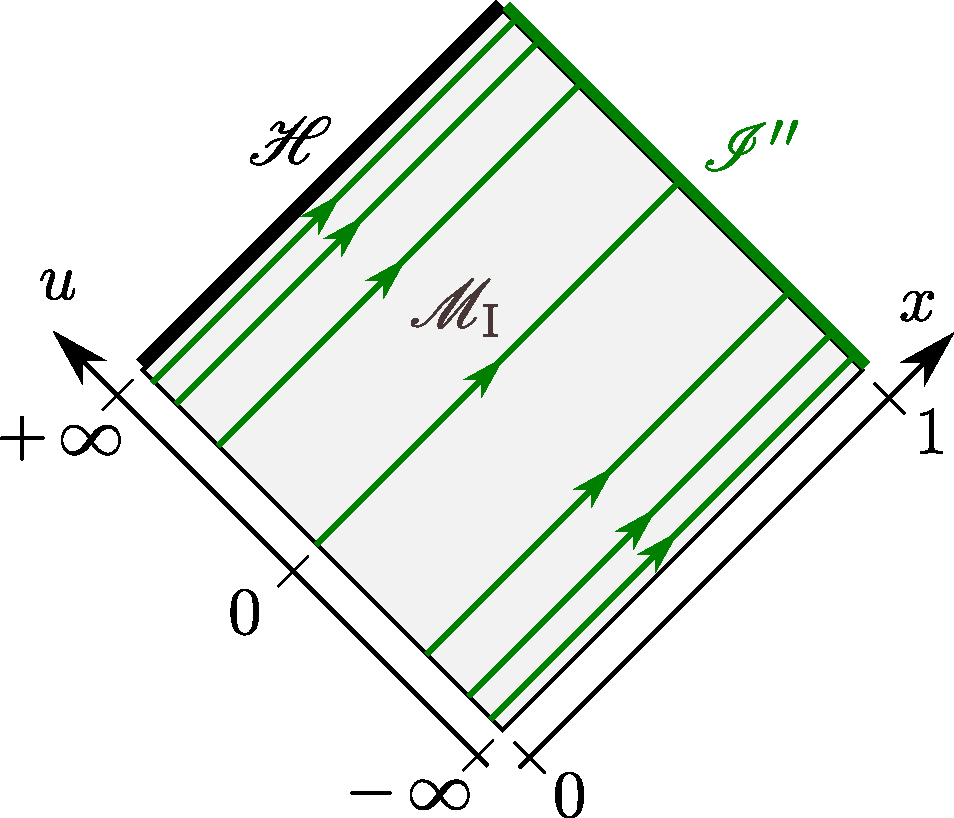
\includegraphics[width=0.4\textwidth]{sch_conf_compl2.pdf}}
\caption[]{\label{f:sch:conf_compl2} \footnotesize
Manifold with boundary
$\M''_{\rm I} = \M_{\rm I}\cup\scri''$, drawn in terms of
the coordinates $x$ and (a compactified version of) $u$.
The green solid lines are the outgoing radial null geodesics (as in Fig.~\ref{f:sch:rad_null_geod_EF}), the arrows marking the future orientation.
Note that $\Hor$, which is drawn on this figure, is not part of $\M''_{\rm I}$.}
\end{figure}

On $\M_{\rm I}$, let us perform the change of coordinates
$(\check{x}^\alpha) = (u,r,\th,\ph) \rightarrow ({x''}^\alpha) = (u,x,\th,\ph)$,
where $x$ is related to $r$ by the same formula as (\ref{e:sch:x_r}),
except that on $\M_{\rm I}$, $x$'s range is $(0,1)$ only.
We deduce from (\ref{e:sch:g_u_r}) and (\ref{e:sch:x_r})
the expression of $\w{g}$ in terms of the coordinates $(u,x,\th,\ph)$:
\be \label{e:sch:tilde_g_x_u}
        {g''}_{\mu\nu}\, \D {x''}^\mu \, \D {x''}^\nu =
            -x \, \D u^2
            -\frac{4 m}{(1-x)^2} \, \D u \, \D x
        + \frac{4 m^2}{(1-x)^2}  \left( \D\th^2 + \sin^2\th\, \D\ph^2 \right) .
\ee
Let us identify $\M_{\rm I}$ with the following open subset of
$\R^2\times \SS^2$:
\be
    \M_{\rm I} = \R \times (0,1) \times \SS^2 ,
\ee
with $u$ spanning $\R$, $x$ spanning $(0,1)$ and $(\th,\ph)$
spanning $\SS^2$. Similarly to what we did above for $\M$, we may then
extend $\M_{\rm I}$ to the manifold with boundary
\be
    \M''_{\rm I} :=  \R \times (0,1] \times \SS^2 .
\ee
The boundary of $\M''_{\rm I}$, $\scri''$ say, lies at $x=1$
(cf. Fig.~\ref{f:sch:conf_compl2}). It shall not be
confused with the boundary of $\M_{\rm I}$ as a submanifold of $\M'$, which is
$\scri'$. The difference arises from the fact that $u$ diverges (to $-\infty$)
when one approaches $\scri'$ in $\M'$, so that $u$ cannot be used as a
coordinate on $\M'$. This is clear on the relation (\ref{e:sch:v_r_u})
between $u$, $v$ and $r$, which, once re-expressed in terms of $x$, becomes
\be \label{e:sch:u_v_x}
    u = v - 4m\left[ \frac{1}{1-x} + \ln\left( \frac{x}{1-x} \right) \right].
\ee
For a fixed value of $v$ in $\M'$, this relation yields diverging values of
$u$ at two places:
\begin{itemize}
\item $x\rightarrow 0^+$ (the horizon $\Hor$): $u\rightarrow +\infty$;
\item $x\rightarrow 1^-$ (the boundary $\scri'$): $u\rightarrow -\infty$.
\end{itemize}
Reciprocally, for a fixed value of $u$, relation~(\ref{e:sch:u_v_x})
implies that $v$ diverges (to $+\infty$) when $x\rightarrow 1^-$, which shows that
$\scri''$ is not included in $\M'$.

The conformal completion of $(\M,\w{g})$ including both $\scri'$ (as $\scri^-$)
and $\scri''$ (as $\scri^+$) is constructed as follows. Let
\be
    \tilde{\M} = \M' \cup \M''_{\rm I} .
\ee
We endow $\tilde{\M}$ with two coordinate charts:
\be
    \begin{array}{rccl}
        \Phi_1: & \M' & \longrightarrow &   \R \times (-\infty,1] \times \SS^2 \\
        & p & \longmapsto & (v,x,\th,\ph) \\[1ex]
    \end{array}
    \qquad\mbox{and}\qquad
    \begin{array}{rccl}
        \Phi_2: & \M''_{\rm I}  & \longrightarrow & \R \times (0,1] \times \SS^2 \\
        & p & \longmapsto & (u,x,\th,\ph)
    \end{array}
\ee
and define the intersection of the two chart codomains:
\be
   \M' \cap  \M''_{\rm I} = \{ p \in \M',\  x(p) \in (0,1) \}
      = \{ p \in \M''_{\rm I},\  x(p) \in (0,1) \} ,
\ee
along with the transition map implementing (\ref{e:sch:u_v_x}):
\be
    \begin{array}{rccl}
        \Phi_2 \circ \Phi_1^{-1}: & \R \times (0,1) \times \SS^2  & \longrightarrow & \R \times (0,1) \times \SS^2 \\
        & (v,x,\th,\ph) & \longmapsto & \left(u = v - 4m\left[ \frac{1}{1-x} + \ln\left( \frac{x}{1-x} \right) \right],\; x,\; \th,\; \ph \right) ,
    \end{array}
\ee
The above construction makes $\tilde{\M}$ a manifold with boundary
(cf. Fig.~\ref{f:sch:conf_compl_final}), the boundary
being
\be
    \scri = \scri^+ \cup \scri^- ,
\ee
with
\be
    \scri^+ := \{ p \in \M''_{\rm I}, \  x(p) = 1 \}
     \qquad\mbox{and}\qquad
    \scri^- := \{ p \in \M', \ x(p) = 1 \} .
\ee

\begin{figure}
\centerline{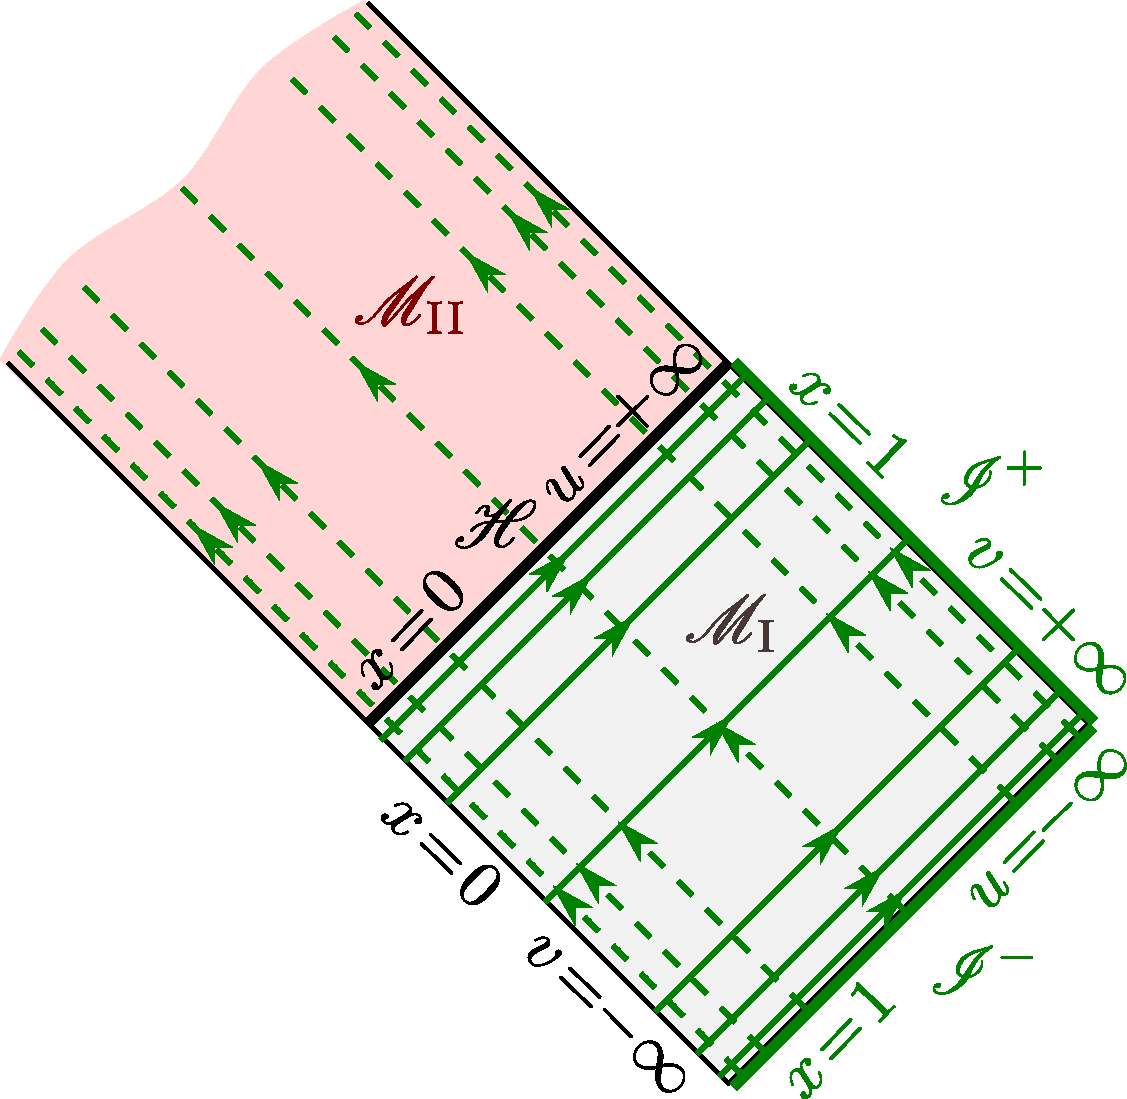
\includegraphics[width=0.5\textwidth]{sch_conf_compl_final.pdf}}
\caption[]{\label{f:sch:conf_compl_final} \footnotesize
Schematic view of the manifold with boundary $\tilde{M}$, which defines
a conformal completion at null infinity of Schwarzschild spacetime
$(\M,\w{g})$.
\emph{NB:} contrary to Figs.~\ref{f:sch:conf_compl1} and~\ref{f:sch:conf_compl2}, this figure is not drawn on some specific coordinate system.
As in Figs.~\ref{f:sch:rad_null_geod_EF}, \ref{f:sch:conf_compl1} and~\ref{f:sch:conf_compl2},
the green solid (resp. dashed) lines are the outgoing (resp. ingoing) radial null geodesics, the arrows marking the future orientation.
}
\end{figure}


We then endow $\tilde{\M}$ with a Lorentzian metric $\w{\tilde{g}}$, whose
expression is given by (\ref{e:sch:tilde_g_x_v}) on $\M'$ and
by (\ref{e:sch:tilde_g_x_u}) on $\M''_{\rm I}$.
By construction, $(\tilde{\M},\w{\tilde{g}})$ is then a conformal completion at null
infinity of the Schwarzschild spacetime $(\M,\w{g})$, the conformal factor
$\Omega$ being given by (\ref{e:sch:Omega_x_r}) in both
charts $(\M',\Phi_1)$ and $(\M''_{\rm I},\Phi_2)$: $\Omega = 1 -x$.
In particular, it is clear that no past-directed causal curve originating in
$\M$ intersects $\scri^+$ and that no future-directed causal curve originating in
$\M$ intersects $\scri^-$. We also check immediately that $\scri^+$ and $\scri^-$
are null hypersurfaces with respect to the metric $\w{\tilde{g}}$:
both hypersurfaces are defined by $x=1$, so that the induced metric on them,
as
deduced from (\ref{e:sch:tilde_g_x_v}) and
(\ref{e:sch:tilde_g_x_u}), is
\be
    \left. \w{\tilde{g}} \right| _{\scri^\pm} = 4 m^2 \left(
        \dd \th\otimes \dd \th + \sin^2\th \, \dd \ph \otimes \dd \ph \right) ,
\ee
which is clearly degenerate (along the $u$ direction for $\scri^+$
and along the $v$ direction for $\scri^-$).

As it is clear from Fig.~\ref{f:sch:conf_compl_final}, $\M_{\rm I}$
is the interior of the causal past of $\scri^+$ within $\M$:
\be
    \M_{\rm I} = \mathrm{int}\left( J^-(\scri^+)\cap\M \right).
\ee
In view of the formal definition (\ref{e:glo:def_BH}), we conclude that
the Schwarzschild spacetime $(\M=\M_{\rm IEF}, \w{g})$
has a black region $\mathscr{B}$, the interior
of which is $\M_{\rm II}$, the event horizon being nothing but the
Schwarzschild horizon $\Hor$.

\begin{remark}
As stated at the beginning of this section, the null character of the boundary
$\Hor$ between $\M_{\rm I}$ and $\M_{\rm II}$ and the fact that
$\M_{\rm II}$ never intersect the asymptotically flat region $r\rightarrow +\infty$,
was sufficient to claim that $\M_{\rm II}$ is what should be
called a \emph{black hole}  of Schwarzschild spacetime.
Therefore, one could view the above demonstration more as a ``sanity'' check
of the formal definition of a black hole given in Sec.~\ref{s:glo:def_BH}.
\end{remark}

\begin{remark}
The above construction of the conformal completion at null infinity
$(\tilde{\M},\w{\tilde{g}})$ involves two coordinate charts,
$(v,x,\th,\ph)$ and $(u,x,\th,\ph)$, with two different (albeit overlapping)
domains.
As will be discussed in Chap.~\ref{s:max},
one may construct a conformal completion
with a single chart, as in the Minkowski case, but its relation with
the coordinate introduced so far is quite involved.
In particular the standard compactification of Kruskal-Szekeres coordinates,
which yield to the Carter-Penrose diagrams as discussed in Sec.~\ref{s:max:Carter-Penrose} below, do \emph{not} provide a
conformal completion of Schwarzschild spacetime.
\end{remark}



